\section{Реализация решения}\label{chapter3}

В главе \ref{chapter2} было представлено описание решения, которое позволит получить промежуточные состояния потока между вызовами промежуточных операций. Чтобы применить решение на практике реализуем расширение для среды разработки IntelliJ IDEA. 

IntelliJ IDEA -- среда для разработки, основанная на платформе IntelliJ, позволяет разрабатывать программы на нескольких языках программирования, в том числе на java. Функциональность платформы может быть расширена с помощью плагинов, которые могут быть установлены из официального репозитория \cite{jb:plugins}, либо из других источников. Платформа предоставляет разработчикам плагинов API -- классы и интерфейсы, с помощью которых компоненты плагина могут быть интегрированы.
\subsection{Нахождение подходящего вызова}

Для нахождения границ вызова будем использовать API, предоставляемый платформой для работы с исходным кодом. Исходный код представлен в виде $AST$-дерева. Обходя его, можно найти цепочки вызовов. Интерфейс платформы позволяет определить тип объекта, на котором вызывается метод и тип результата вызова. Используя следующие правила, мы сможем классифицировать вызовы внутри цепочки:
\begin{itemize}
	\item Промежуточный - вызов возвращающий объект, реализующий \mintinline{java}{Stream<T>}.
	\item Завершающий - вызов на объекте, реализующем \mintinline{java}{Stream<T>}, возвращающий объект произвольного типа, не реализующем \mintinline{java}{Stream<T>}. 
\end{itemize}

Учитывая, что положение отладчика может быть отображено на некоторый элемент $AST$-дерева, у нас есть возможность обойти поддерево этого элемента и найти все подходящие цепочки. Кроме того, мы не привязываемся к именам методов для промежуточных операций, это снижает требование к потоку, который может быть отлажен (вызовы с неподдерживаемым операциями могут отлаживаться: для них будут построены состояния, но переходы восстановить не удастся). Таким образом, можно удовлетворить всем требованиям из \ref{detection}.

Отдельно стоит рассмотреть редкий случай, когда результат завершающей операции наследник \mintinline{java}{Stream<T>}. Действуя неосторожно, можно перепутать такую завершающую операцию с промежуточной. Чтобы этого избежать, необходимо проверить, что имя операции не совпадает с именами терминальных операций, которые могут вернуть \mintinline{java}{Stream<T>}. Таких операций немного -- \mintinline{java}{collect} и \mintinline{java}{reduce}.

\subsection{Построение выражения}
Во второй главе был получен важный результат. Для того, чтобы восстановить все переходы, их нужно восстановить локально для каждого из промежуточных вызовов. При этом необходимая информация для построения переходов у разных операций может различаться. Поэтому будет удобно добавить абстракции, которые позволят каждому вызову модифицировать цепочку, чтобы собрать данные для восстановления переходов. 

Но для всех вызовов верно, что они требуют лишь локальной модификации цепочки: добавления методов до и после самого вызова. 

Таким образом, достаточно ввести абстракции, которые позволят:
\begin{itemize}
	\item Объявить локальные переменные в выражении для вычисления, нужные для сохранения информации о вычислении.
	\item Добавить промежуточные вызовы в цепочку до и после самой операции.
	\item Преобразовать собранную информацию в процессе запуска выражения к удобному представлению для дальнейшей интерпретации.
\end{itemize}

При этом, нужно позаботиться, чтобы имена локальных переменных, которые используют разные вызовы были различны. Самый простой способ этого достичь - добавить к имени используемых переменных номер вызова.

Упрощенно, структура фрагмента кода для вычисления с точки зрения одной операции будет выглядеть следующим образом:

\inputminted{java}{chapter3/code/EvalCode.java}

Пример сгенерированного кода есть в приложении А.

\subsection{Вычисление выражения}
В \ref{code-evaluation} описаны подходы к вычислению произвольного кода внутри отладчика. Там же был сделан выбор в пользу стратегии загрузки и запуска новых классов. Данная возможность уже присутствует в среде разработки, поэтому не будем подробно останавливаться на деталях реализации этого процесса. У такого подхода есть недостаток -- у загружаемых классов может не быть прав доступа в некоторым полям и методам других объектов. Это происходит из-за того, что новый класс компилируется как внутренний класс для класса, внутри которого находится отладчик при запуске операции вычисления выражения. Но класс, в котором находится отладчик уже загружен, и он не знает о новом внутреннем классе, поэтому не может предоставить доступ к приватным полям и методам.

Для решения этой проблемы используется внутренний класс JDK \\ \mintinline{java}{MagicAccessorImpl} \cite{magic}. Это часть небезопасного API java. Наследование от этого класса является маркером для виртуальной машины java, что необходимо пропустить проверки доступа при вызове методов и обращении к полям из методов класса-наследника \mintinline{java}{MagicAccessorImpl}.

Кроме сгенерированного класса, анонимные функции тоже могут пытаться получить доступ к приватным методам и полям. В текущей версии платформы это приведет к исключению. Но это можно обойти, преобразовав все анонимные функции, которые встречаются в выражении, в анонимные классы, которые наследуются от \mintinline{java}{MagicAccessorImpl}. Для этого преобразования можно использовать существующие рефакторинги для преобразования анонимных функций в анонимные классы.

Таким образом, весь код внутри нашего выражения для построения состояний и переходов не будет иметь проблем с доступом к методами и полям других классов.

\subsection{Визуализация}
После завершения вычисления у нас имеется набор промежуточных состояний и переходы между ними. Промежуточные состояния -- это не просто список объектов. Переходы -- это связь между объектам в двух соседних состояниях. Наиболее естественно это визуализировать с помощью двух списков объектов и линий-переходов.

При выборе какого-либо значения в списке нужно визуально выделить все объекты, с которыми он связан, затем те, с которыми связаны они и т.д. 

В результате был разработан следующий интерфейс:

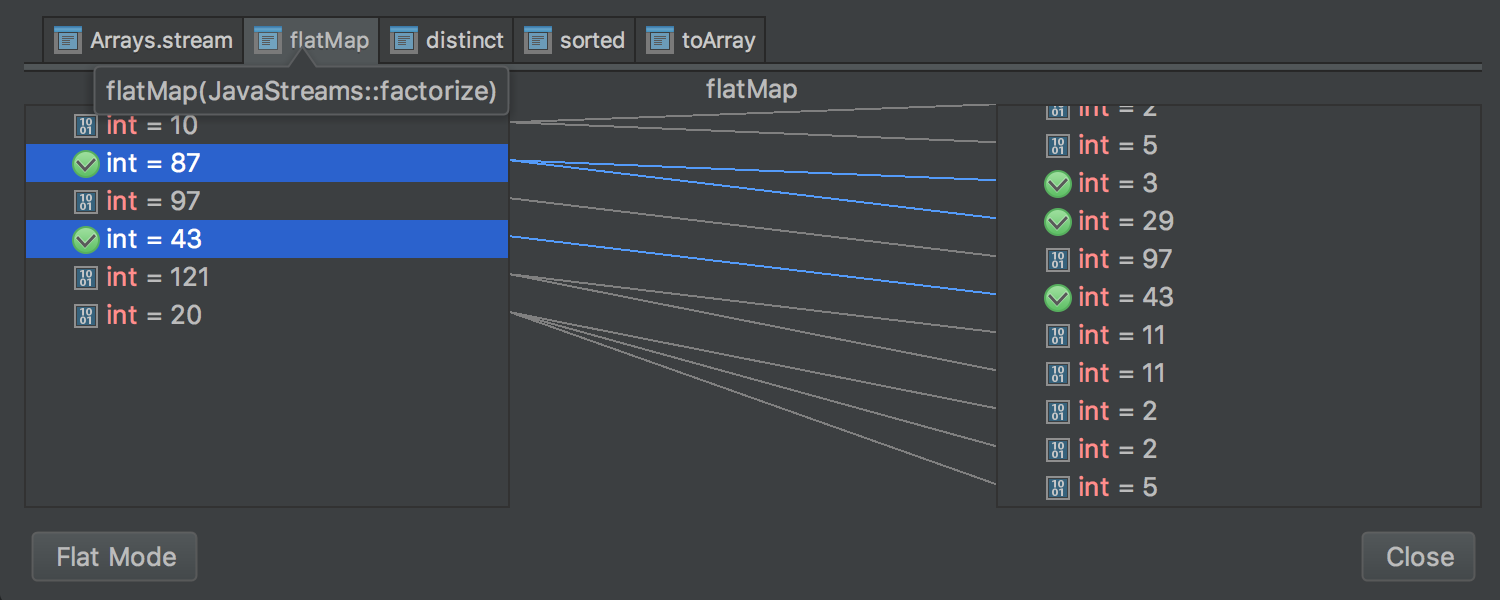
\includegraphics[scale=0.25]{chapter3/img/split-view.png}

Дополнительно, есть возможность просмотреть всю цепочку целиком:

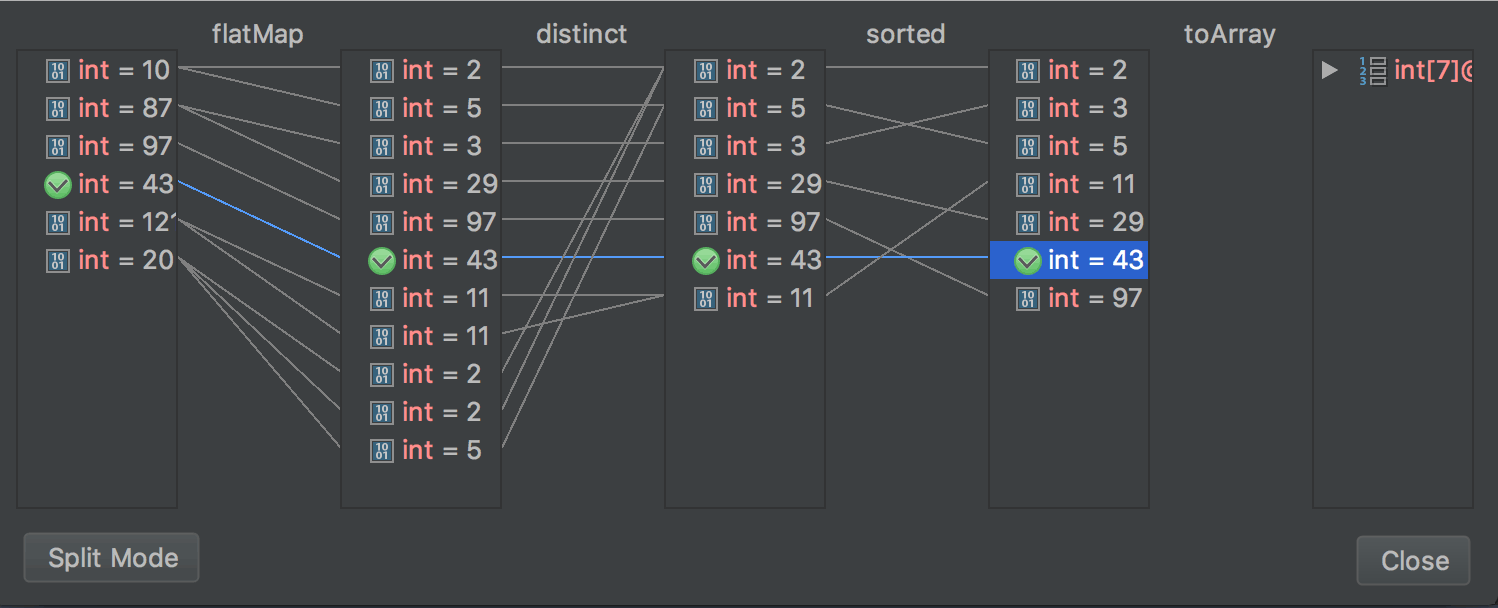
\includegraphics[scale=0.36]{chapter3/img/flat-view.png}










